% Prototype configuration: the path selected from the domain feature model.
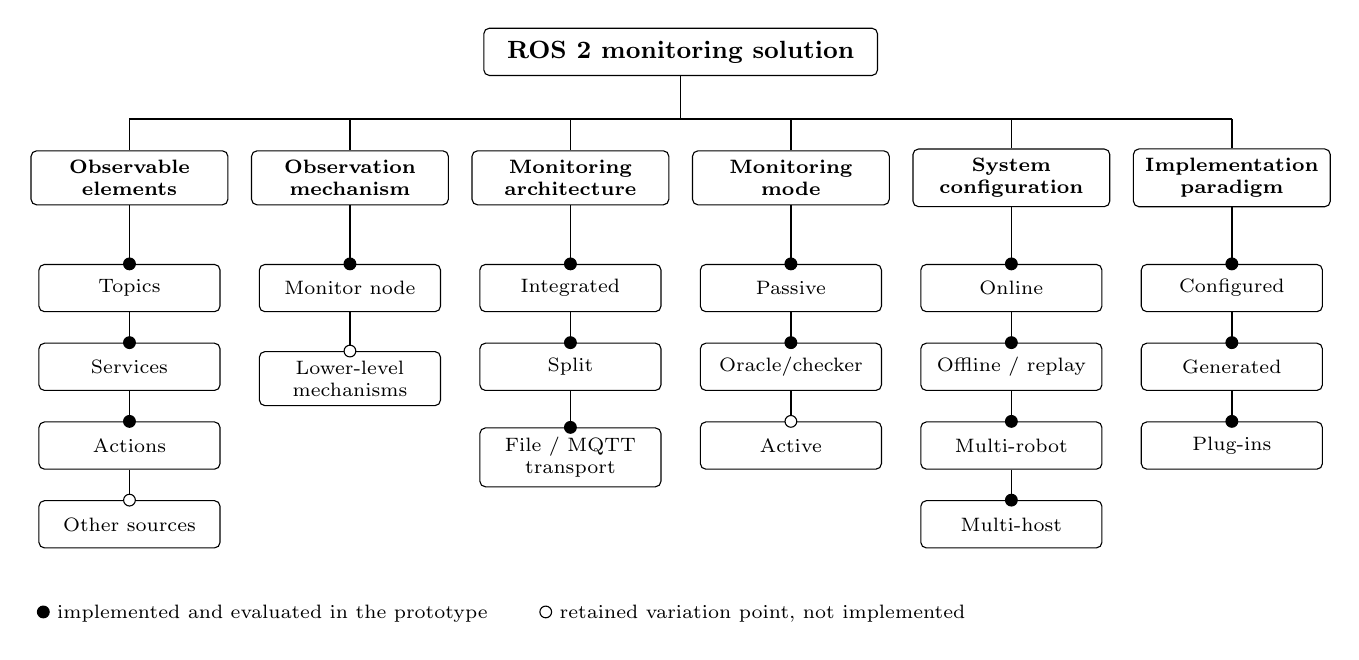
\begin{tikzpicture}[
  font=\scriptsize,
  feature/.style={draw, fill=white, rounded corners=2pt,
                  align=center, minimum height=6mm, minimum width=23mm,
                  inner xsep=3pt},
  root/.style={feature, font=\small\bfseries, minimum width=50mm},
  group/.style={feature, font=\scriptsize\bfseries, minimum width=25mm},
  line/.style={draw, line width=.6pt},
  selected/.style={circle, draw, fill=black, inner sep=1.5pt},
  unselected/.style={circle, draw, fill=white, inner sep=1.5pt}
]
\node[root] (root) at (0,0) {ROS 2 monitoring solution};

% group row
\node[group] (elements) at (-7.0,-1.6) {Observable\\elements};
\node[group] (mech) at (-4.2,-1.6) {Observation\\mechanism};
\node[group] (arch) at (-1.4,-1.6) {Monitoring\\architecture};
\node[group] (mode) at (1.4,-1.6) {Monitoring\\mode};
\node[group] (config) at (4.2,-1.6) {System\\configuration};
\node[group] (paradigm) at (7.0,-1.6) {Implementation\\paradigm};

% root -> horizontal bus -> groups (bus above all group boxes)
\draw[line] (root.south) -- (0,-0.85);
\draw[line] (-7.0,-0.85) -- (7.0,-0.85);
\foreach \n in {elements,mech,arch,mode,config,paradigm}
  \draw[line] (\n.north |- 0,-0.85) -- (\n.north);

% column: observable elements
\node[feature] (topic) at (-7.0,-3.0) {Topics};
\node[feature] (service) at (-7.0,-4.0) {Services};
\node[feature] (action) at (-7.0,-5.0) {Actions};
\node[feature] (other) at (-7.0,-6.0) {Other sources};

% column: observation mechanism
\node[feature] (monnode) at (-4.2,-3.0) {Monitor node};
\node[feature] (lowlevel) at (-4.2,-4.15) {Lower-level\\mechanisms};

% column: architecture
\node[feature] (integrated) at (-1.4,-3.0) {Integrated};
\node[feature] (split) at (-1.4,-4.0) {Split};
\node[feature] (transport) at (-1.4,-5.15) {File / MQTT\\transport};

% column: monitoring mode
\node[feature] (passive) at (1.4,-3.0) {Passive};
\node[feature] (oracle) at (1.4,-4.0) {Oracle/checker};
\node[feature] (active) at (1.4,-5.0) {Active};

% column: system configuration
\node[feature] (online) at (4.2,-3.0) {Online};
\node[feature] (offline) at (4.2,-4.0) {Offline / replay};
\node[feature] (multirob) at (4.2,-5.0) {Multi-robot};
\node[feature] (multihost) at (4.2,-6.0) {Multi-host};

% column: implementation paradigm
\node[feature] (configured) at (7.0,-3.0) {Configured};
\node[feature] (generated) at (7.0,-4.0) {Generated};
\node[feature] (plugins) at (7.0,-5.0) {Plug-ins};

% vertical chains inside each column
\foreach \a/\b in {elements/topic, topic/service, service/action,
                   action/other,
                   mech/monnode, monnode/lowlevel,
                   arch/integrated, integrated/split, split/transport,
                   mode/passive, passive/oracle, oracle/active,
                   config/online, online/offline, offline/multirob,
                   multirob/multihost,
                   paradigm/configured, configured/generated,
                   generated/plugins}
  \draw[line] (\a.south) -- (\b.north);

% selection markers on the top edge of each feature box
\foreach \n in {topic,service,action,monnode,integrated,split,transport,
                passive,oracle,online,offline,multirob,multihost,
                configured,generated,plugins}
  \node[selected] at (\n.north) {};
\foreach \n in {other,lowlevel,active}
  \node[unselected] at (\n.north) {};

% legend
\node[anchor=north west, align=left, font=\scriptsize] at (-8.3,-6.9) {%
  \tikz\node[selected]{};\ implemented and evaluated in the prototype
  \qquad
  \tikz\node[unselected]{};\ retained variation point, not implemented};
\end{tikzpicture}
